%
% LaTeX-Template for Master Theses
%	 @ FH Kaernten
%
% V 1.0
% Feb. 2011
% M.Koeberle
%
% Example Chapter 2
%

\chapter{Automated Material Handling in Semiconductor Factories}
\label{cha:AMH}



\section{Wafers and Carriers}
\label{sec:WaferCarrier}

A semiconductor factory can have a total building area of around 60.000 m$^2$ which results in a clean room area of roughly 20.000 m$^2$ \cite{InfineonTechnologiesAG.17.07.2023}. In this clean room area the semiconductors are manufactured on substrates, the so called wafers. In Figure \ref{fig:300mmThinWafer} a 300 mm thin wafer which is produced in the new factory of Infineon can be seen.

\begin{figure}[h]
    \centering
    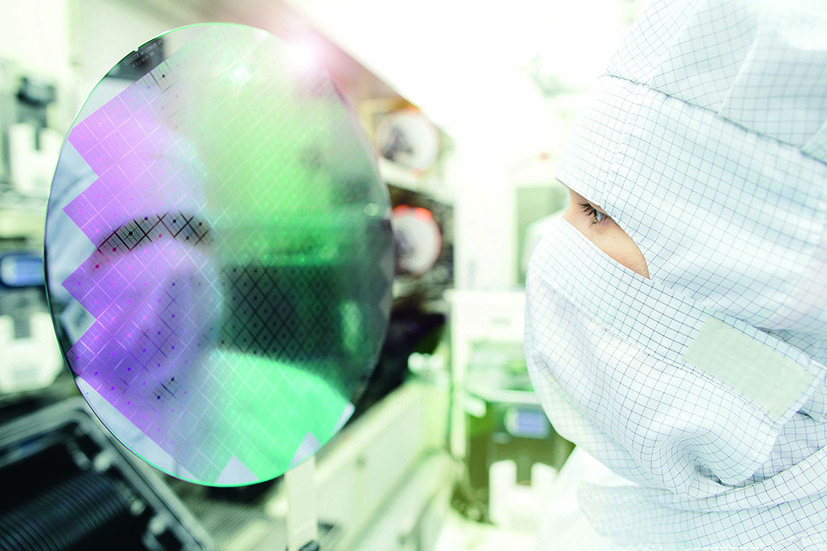
\includegraphics[scale=2.0]{pictures/Infineon-Chipfab-Thin-Wafer-300-mm-Villach.jpg}
    \caption{300 mm Thin Wafer from Infineon \cite{300mmThinWafer.17.09.2021}}
    \label{fig:300mmThinWafer}
\end{figure}

Each wafer starts as a raw and thin disc made out of silicon and is then transformed into integrated circuits. This transformation procedure typically contains between 300 and 700 processing steps that take place on more than 100 manufacturing equipments \cite{monch2012production}. For safer and easier transportation the $\sim$775 μm thick wafers are packed into carriers \cite{Wikipedia.2024}. For the 300 mm wafers the most common type of carrier is the front opening unified pod (\gls{foup}) which can be seen in Figure \ref{fig:Foup}.

\begin{figure}[h]
    \centering
    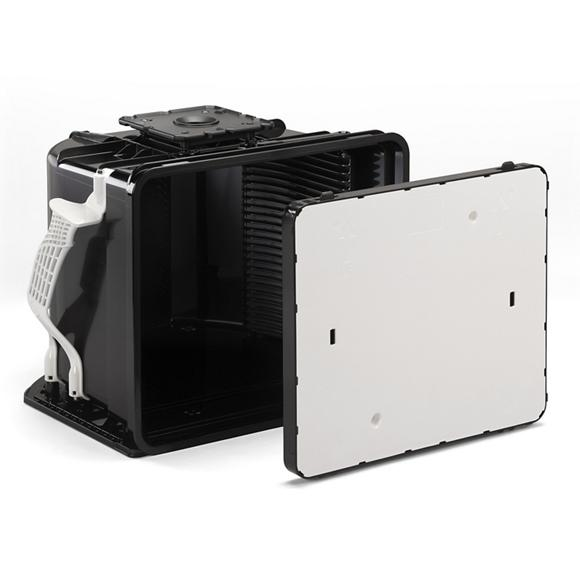
\includegraphics[scale=0.5]{pictures/product-a300g3foupwafercarriers-1-2.jpeg}
    \caption{A300 G3 \gls{foup} Wafer Carrier from Entegris \textbf{Source Needed!!!}} %https://www.entegris.com/shop/en/USD/products/wafer-handling/wafer-processing/300-mm-front-opening-unified-pods-%28foups%29/A300-FOUPs/p/A300FOUPs Quelle hinzufügen
    \label{fig:Foup}
\end{figure}

In a semiconductor plant more than 10,000 carriers are commonly present. One process step has a duration range from a few minutes to 24 hours. The carriers have to be moved between the processes and also the storage. It is important to mention that a \gls{foup} that is waiting to be picked up from the equipment is blocking the loadport of the equipment. On the other hand, an equipment waiting for a new \gls{foup} is not active and therefore does not generate revenue. The transport times between the different manufacturing equipments and storage have to be minimized in order to guarantee high utilization of the equipment. A full \gls{foup} with 25 wafers weighs approximately 9 kg \cite{ManualFoupHandling} and has to be transported between a few meters and more than 200 m. The repeated labour of manual transportation of the \gls{foup}s has been associated with musculoskeletal disorders in human wafer handlers. It is therefore clear that this work should be automated, both from an occupational safety and an economic point of view \cite{ManualFoupHandling}.\newpage

\section{Automated Material Handling (\gls{amh})}
\label{sec:AMH}
Automated Material Handling (\gls{amh}) describes the automated transportation and storage of material in a manufacturing plant. The \gls{foup}s as carriers represent the material that has to be transported in this case. The carriers that are transported or stored in the factory are located in the automated material handling system (\gls{amhs}). The term automated material handling is standardized by the semiconductor equipment and materials international (SEMI) standard through standard documents that are published in the SEMI standard. SEMI is an association of more than 2000 companies world wide active in the electronics design and manufacturing supply chain. Today more than 1000 standards related to electronics are developed and maintained by this association \cite{SEMI}\cite{Semi.org}.


\section{Overhead Hoist Transport (OHT) System}
\label{sec:OHT}


\newpage